\documentclass{article}
\usepackage[utf8]{inputenc}
\usepackage{graphicx}
\usepackage{amsmath }
\usepackage{amssymb}
\usepackage{subcaption}
\usepackage{float}


\usepackage{cleveref} %referencing figures, equations and tables
\crefformat{figure}{Figure.~#2#1#3}
\crefformat{equation}{Eq.~#2#1#3}
\crefformat{table}{Table.~#2#1#3}
\crefformat{appendix}{Appendix.~#2#1#3}
\crefformat{section}{Section.~#2#1#3}

\title{Wave Propagation in a Cantilever Beam Under Normal Load}
\author{Amir Baharvand }
\date{}

\begin{document}

\maketitle

\subsection{Applied Load in Form of a Step Function}

The problem description is provided in \cite{ACHENBACH:1975} (problem 8.1).

\subsection{Problem Statement}
The one-dimensional wave equation can be expressed in the form of

\begin{equation}
    \dfrac{\partial^2 u}{\partial t^2} = c^2 \dfrac{\partial^2 u}{\partial x^2}
    \label{eq:wave_eqn}
\end{equation}

where $x$ and $t$ denote position and time. $u$ is the displacement and is a function of both $x$ and $t$ and $c$ is the velocity of wave propagation. For the problem under study, which is the wave propagation in a cantilever beam under normal stress, the initial and boundary conditions (I.C and B.C) are defined as below.

\begin{equation*}
\begin{matrix}
    \text{I.C}\begin{cases}
        u(x, 0) = 0 \\ 
        \\
        \dfrac{\partial u(x, 0)}{\partial t} = 0 
    \end{cases} \quad , \quad
    \text{B.C}\begin{cases}
        u(0, t) = 0 \\
        \\
        \dfrac{\partial u(L, t)}{\partial x} = \dfrac{P(t)}{EA}
    \end{cases}
\end{matrix}
\end{equation*}

In the above equations, $L$ is the length, $P(t)$ is the applied force at the right end of the beam, $E$ is the Young's modulus and $A$ is the cross-sectional area of the beam (\cref{fig:beam}).

\begin{figure}[H]
    \centering
    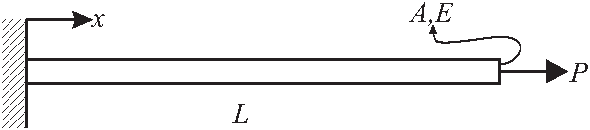
\includegraphics[width = 0.6\textwidth ]{figures/beam.pdf}
    \caption{Cantilever beam geometry, boundary condition and coordinate system.}
    \label{fig:beam}
\end{figure}

\section{Applied Load in Form of the Step Function}
Applying the load in form of the step function, $H(t)$, requires modification of B.C accordingly, that is 

\begin{equation*}
    \text{B.C}\begin{cases}
        u(0, t) = 0 \\
        \\
        \dfrac{\partial u(L, t)}{\partial x} = \dfrac{P H(t)}{EA}
    \end{cases}
\end{equation*}

The rest of the problem remains intact.

\subsection{Solving the Wave Equation Using Fourier Series}
In the following section, the solution to the wave equation using the Fourier series is presented. Due to the inhomogeneity of B.C, it is essential to convert the initial problem into another one with a homogeneous B.C, then by invoking the separation of variables method and superposition of generated Fourier series, the final Partial Differential Equation (PDE) is solved.

\subsubsection{Step 1: Converting B.C to homogeneous conditions}
First, it is assumed that the solution of the wave equation, $u(x, t)$, can be written in form of two functions, $w$ and $v$ as below.

\begin{equation}
    u(x, t) = w(x, t) + v(x) \Rightarrow \begin{cases}
        \dfrac{\partial^2 u}{\partial x^2} = \dfrac{\partial^2 w}{\partial x^2} + v''(x) \\
        \\
        \dfrac{\partial^2 u}{\partial t^2} = \dfrac{\partial^2 w}{\partial t^2}
    \end{cases}
\label{eq:nh2h}
\end{equation}

Substituting \cref{eq:nh2h} in \cref{eq:wave_eqn} gives

\begin{equation}
    \dfrac{\partial^2 w}{\partial t^2} = c^2 \left[ \dfrac{\partial^2 w}{\partial x^2} + v''(x) \right]
\label{eq:trans_wave_eqn}
\end{equation}

Next, it is assumed that $v''(x)$ is zero; therefore, $v(x) = ax + b$ and the B.C becomes

\begin{equation*}
\begin{matrix}
    \text{B.C}\begin{cases}
        u(0, t) = 0 \\
        \\
        \dfrac{\partial u(L, t)}{\partial x} = \dfrac{P(t)}{EA}
    \end{cases}
    \Rightarrow
    \begin{cases}
        w(0, t) + v(0) = 0 \\
        \\
        \dfrac{\partial w(L, t)}{\partial x} + v'(L) = \dfrac{P(t)}{EA}
    \end{cases}
\end{matrix}
\end{equation*}

where by assuming that both $w(0, t)$ and $\dfrac{\partial w(L, t)}{\partial x}$ to be zero in the above equation, $a = \dfrac{P(t)}{EA}$ and $b= 0$. As a result, $v(x) = \dfrac{P(t)}{EA} x$.

Then, we determine $w(x, t)$. \cref{eq:trans_wave_eqn} reduces to 

\begin{equation}
    \dfrac{\partial^2 w}{\partial t^2} = c^2 \dfrac{\partial^2 w}{\partial x^2}
\label{eq:red_trans_wave_eqn}
\end{equation}

with the following I.C and B.C

\begin{equation*}
\begin{matrix}
    \text{I.C}\begin{cases}
        w(x, 0) + v(x)= 0 \\ 
        \\
        \dfrac{\partial w(x, 0)}{\partial t} = 0 
    \end{cases}
    \Rightarrow 
    \begin{cases}
        w(x, 0) = \dfrac{-P(t)}{EA}x \\ 
        \\
        \dfrac{\partial w(x, 0)}{\partial t} = 0 
    \end{cases} \quad , \quad
    \text{B.C}\begin{cases}
        w(0, t) = 0 \\
        \\
        \dfrac{\partial w(L, t)}{\partial x} = 0
    \end{cases}
\end{matrix}
\end{equation*}

Hence, the original PDE with the inhomogeneous B.C is converted into another PDE with homogeneous B.C

\subsubsection{Step 2: Using the separation of variables method}
To solve the generated PDE from previous section (\cref{eq:red_trans_wave_eqn}), we assume

\begin{equation}
\begin{matrix}
    w(x, t) = F(x) G(t) \Rightarrow \begin{cases}
        \dfrac{\partial^2 w}{\partial x^2} = F''(x) G(t) \\
        \\
        \dfrac{\partial^2 u}{\partial t^2} = F(x) \ddot{G}(t)
    \end{cases}
\end{matrix}
\label{eq:vsm}
\end{equation}

where $F''(x) = \dfrac{\partial^2 F(x)}{\partial x^2}$ and $\ddot{G}(t) = \dfrac{\partial^2 G(t)}{\partial t^2}$. By plugging in \cref{eq:vsm} into \cref{eq:red_trans_wave_eqn} and reordering the terms, we have

\begin{equation}
    F(x) \ddot{G}(t) = c^2 F''(x) G(t) \Rightarrow \dfrac{\ddot{G}(t)}{c^2 G(t)} = \dfrac{F''(x)}{F(x)}
\end{equation}

In the above equation, for both sides to be equal, $\dfrac{\ddot{G}(t)}{c^2 G(t)} = \dfrac{F''(x)}{F(x)} = \lambda^2$. Here, $\lambda^2$ can exploit three values: zero, positive and negative.

\paragraph{Case $\lambda^2$ = 0}
For this case, $F''(x) = \lambda^2 F(x)$ reduces to $F''(x) = 0$ which gives $F(x) = Ax + B$. With the given B.C from \cref{eq:red_trans_wave_eqn}, both $A$ and $B$ become zero, which are the trivial solutions. The same can be applied to the equation with $G(t)$.

\paragraph{Case $\lambda^2 >$ 0}
In this case, $F''(x) -\lambda^2 F(x) = 0$ which is an Ordinary Differential Equation (ODE). Using \texttt{dsolve} commnad in Maple, $F(x) = A e^{\lambda x} + B e^{-\lambda x}$. Applying the B.C 

\begin{equation*}
\begin{matrix}
    \begin{cases}
        A + B = 0 \\
        \\
        A e^{\lambda x} - B e^{-\lambda x} = 0
    \end{cases}
\end{matrix}
\end{equation*}

Solving for both $A$ and $B$ results in $A = B = 0$ which is the trivial solution. The same applies to the equation with $G(t)$.

\paragraph{Case $\lambda^2 <$ 0}
Solving the ODE $F''(x) + \lambda^2 F(x) = 0$ gives $F(x) = A \sin(\lambda x) + B \cos(\lambda x)$. After applying the B.C

\begin{equation*}
\begin{matrix}
    \begin{cases}
        B = 0 \\
        \\
        A \lambda \cos(\lambda L) = 0 \quad , \quad
    \end{cases}
\end{matrix}
\end{equation*}

where for the nontrivial solution, 

\begin{equation*}
    \cos(\lambda L) = 0 \Rightarrow \lambda L = n \pi - \frac{\pi}{2} \quad , \quad n = 1, 2, ... \Rightarrow F(x) = A \sin \left[ \dfrac{(2n - 1)\pi}{2L} x \right] \quad , \quad n = 1, 2, ...
\end{equation*}

Following the same steps for the other equation,

\begin{equation*}
    \ddot{G}(t) + c^2 \lambda^2 G(t) = 0 \Rightarrow G(t) = C \sin(c \lambda t) + D \cos(c \lambda t) = 0
\end{equation*}

Applying the I.C from \cref{eq:red_trans_wave_eqn}, $C = 0$ and 

\begin{equation*}
    G(t) = D \cos(c \lambda t) \quad , \quad \lambda = \dfrac{(2n-1)\pi}{2L} \quad , \quad n = 1, 2, ...
\end{equation*}

Therefore, 

\begin{equation}
    w(x, t) = \sum_{n = 1}^{\infty} F(x) G(t) = \sum_{n = 1}^{\infty} Q_n \sin \left[ \dfrac{(2n-1)\pi}{2L} x \right] \cos \left[ \dfrac{(2n-1)\pi}{2L} c t \right]
\end{equation}

$Q_n$ is the product of various terms in both $A$ and $D$ coefficients. By applying the following B.C

\begin{equation*}
    w(x, 0) = \dfrac{-P(t)}{EA} x \Rightarrow \sum_{n = 1}^{\infty} D_n \sin \left[ \dfrac{(2n-1)\pi}{2L} x \right] = \dfrac{-P(t)}{EA} x
\end{equation*}

a Fourier series is generated whereby $Q_n$ can be determined from.

\begin{equation*}
    Q_n = \dfrac{2}{L} \int_{0}^{L} \left(\dfrac{P(t)}{EA} x \right) \sin \left[ \dfrac{(2n-1)\pi}{2L} x \right] dx = \dfrac{8 P(t) L}{AE} \left[ \dfrac{\dfrac{\pi}{2} (2n-1) \sin(\pi n) + \cos(\pi n)}{(2n-1)^2 \pi^2} \right] \quad , \quad n = 1, 2, ...
\end{equation*}

Finally, 

\begin{equation}
\begin{aligned}
    u(x, t)& = w(x, t) + v(x)\\
    &= \sum_{n = 1}^{\infty} \dfrac{8 P(t) L}{AE} \left[ \dfrac{\dfrac{\pi}{2} (2n-1) \sin(\pi n) + \cos(\pi n)}{(2n-1)^2 \pi^2} \right] \cos \left[ \dfrac{(2n-1)\pi}{2L} c t \right] + \dfrac{P(t)}{EA} x \quad , \quad n = 1, 2, ...
\end{aligned}
\end{equation}


\subsubsection{Displacement and Stress Plots}
\cref{fig:u_sigma_sv} shows the normalized longitudinal displacement and stress of the beam for different time increments. As it is seen, the beam experience its maximum elongation after $t= 2$s and this is when the tensile wave has traveled from the right side of the beam (see \cref{fig:beam}), bounced back from the fixed part and again met the right end of the beam. The periodicity is 4s and due to the fixed applied load in terms of a step function, the stress plot is constant for various time increments. 


\begin{figure}[H]
        \begin{subfigure}{0.9\textwidth}
            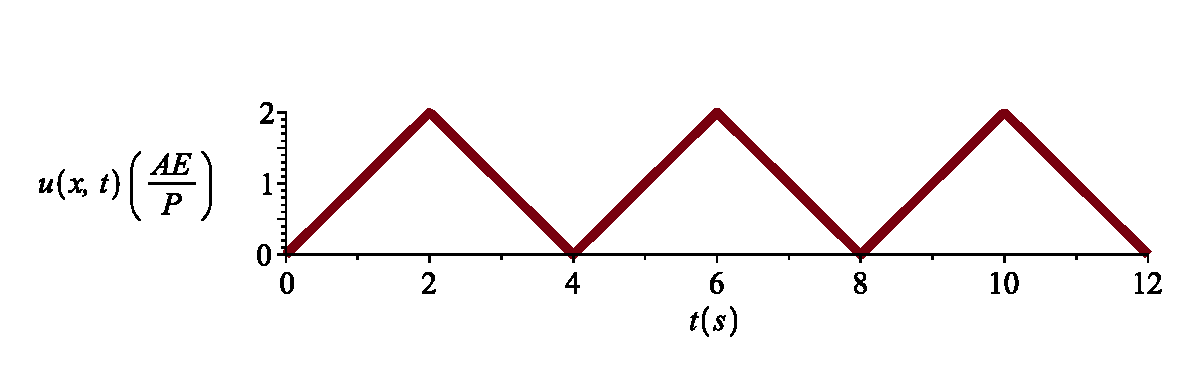
\includegraphics[width=\columnwidth]{figures/a_u_sv.eps} 
            \caption{}
            % \label{}
        \end{subfigure}
        \begin{subfigure}{0.9\textwidth}
            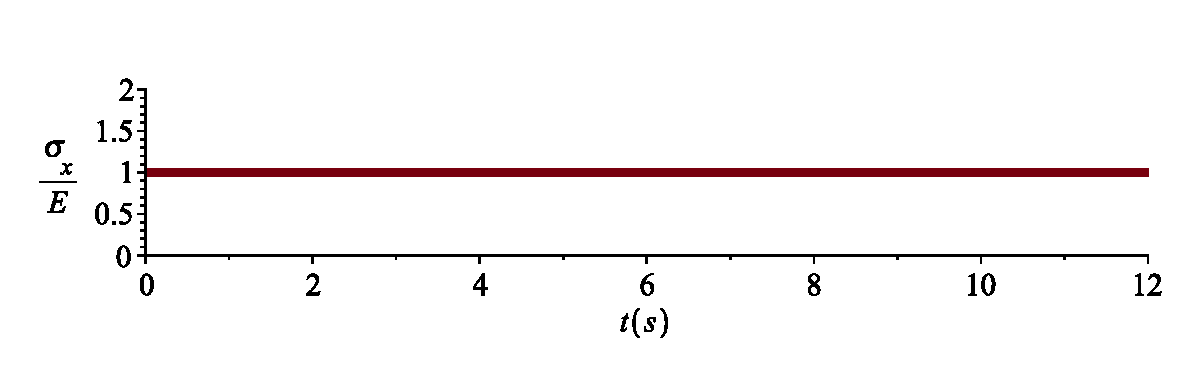
\includegraphics[width=\columnwidth]{figures/a_sigma_sv.eps} 
            \caption{}
            % \label{}
        \end{subfigure}
    \caption{Case $P H(t)$: Normalized longitudinal (a) displacement, $u(x, t)$, and (b) stress, $\sigma_x$, for different time increments($L$, $c$ and $x$ are equal to 1). Number of terms in the series is 1000.}
    \label{fig:u_sigma_sv}
\end{figure}


\subsection{Solving the Wave Equation Using Laplace Transform}

\subsubsection{Using Taylor Series Expansion of $\dfrac{1}{1 - x} = \displaystyle\sum_{n = 0}^{\infty} x^n$}
Let $U(x, s)$ be the Laplace transform ($\mathcal{L}$) of $u(x, t)$

\begin{equation}
    U(x, s) = \mathcal{L}\{u(x, t)\} = \int_{0}^{\infty} u(x, t) e^{-st} dt
    \label{eq:laplace_u}
\end{equation}

In the solution procedure, it is required to calculate the Laplace transform of both $\dfrac{\partial^2 u(x, t)}{\partial x^2}$ and $\dfrac{\partial^2 u(x, t)}{\partial t^2}$ and substitute them in the wave equation (\cref{eq:wave_eqn}). \\

From \cref{eq:laplace_u}

\begin{equation*}
    \dfrac{\partial U(x, s)}{\partial x} = \dfrac{\partial}{\partial x} \int_{0}^{\infty} u(x, t) e^{-st} dt
\end{equation*}

As $u(x, t)$ is the only term on the right-hand of the above equation that is a function of $x$, one is able to move $\dfrac{\partial}{\partial x}$ into the integral, which gives

\begin{equation*}
    \dfrac{\partial U(x, s)}{\partial x} = \int_{0}^{\infty} \dfrac{\partial u(x, t)}{\partial x} e^{-st} dt
\end{equation*}

Similarly,

\begin{equation}
    \dfrac{\partial^2 U(x, s)}{\partial x^2} = \int_{0}^{\infty} \dfrac{\partial^2 u(x, t)}{\partial x^2} e^{-st} dt
    \label{eq:laplace_u_x}
\end{equation}

For the derivation of $\dfrac{\partial^2 u(x, t)}{\partial t^2}$, the following property from Laplace transform is used.

\begin{equation}
    \mathcal{L}\{\dfrac{\partial ^2u(x, t)}{\partial t^2}\} = s^2 \mathcal{L}\{u(x, t)\} - s u(x, 0) - \dfrac{\partial u(x, 0)}{\partial t}
    \label{eq:laplace_prop}
\end{equation}

In the above equation, $s$ is the frequency parameter. According to the given I.C, both the second and third terms on the right-hand side of \cref{eq:laplace_prop} vanish and 

\begin{equation}
    \mathcal{L}\{\dfrac{\partial ^2u(x, t)}{\partial t^2}\} = s^2 \mathcal{L}\{u(x, t)\}
    \label{eq:laplace_u_t}
\end{equation}

Applying Laplace transform on both sides of \cref{eq:wave_eqn} and replacing the relevant terms with the result from \cref{eq:laplace_u_x} and \cref{eq:laplace_u_t} give

\begin{equation}
    s^2 U(x, s) = c^2 \dfrac{\partial^2 U(x, s)}{\partial x^2}
    \label{eq:ode}
\end{equation}

which is an ODE. To solve \cref{eq:ode}, \texttt{dsolve} command from Maple along with the method of Laplace transform and given B.C are utilized. \cref{eq:b_laplace_sch} is the answer from Maple 

\begin{equation}
    U(x, s) = \frac{P(s) c}{AE s} \frac{\sinh(\dfrac{sx}{c})}{\cosh(\dfrac{sL}{c})}
    \label{eq:b_laplace_sch}
\end{equation}

where $P(s)$ is the Laplace transform of load. $\sinh$ and $\cosh$ can be replaced from

\begin{equation*}
    \sinh(x) = \dfrac{e^x - e^{-x}}{2} \quad , \quad \cosh(x) = \dfrac{e^x + e^{-x}}{2}
\end{equation*}

which gives 

\begin{equation}
    U(x, s) = \frac{P(s) c}{AE s} \frac{e^{\frac{sx}{c}} - e^{-\frac{sx}{c}}}{e^{\frac{sL}{c}} + e^{-\frac{sL}{c}}}
    \label{eq:b_laplace_e}
\end{equation}

In order to find the Laplace inverse of $U(x, s)$, which is the solution to $u(x, t)$, first, we need to simplify \cref{eq:b_laplace_e}.

\begin{equation}
    U(x, s) = \frac{P(s) c}{AE s} \frac{e^{s(\frac{L}{c} + \frac{x}{c})} - e^{s(\frac{L}{c}-\frac{x}{c})}}{e^{2\frac{sL}{c}} + 1}
    \label{eq:b_laplace_e1}
\end{equation}

Next, from the Taylor expansion of $\dfrac{1}{1 - x} = \displaystyle\sum_{n = 0}^{\infty} x^n$, we are able to rewrite the denominator in the previous equation.

\begin{equation*}
    \frac{1}{1 - (-e^{\frac{2sL}{c}})} = \sum_{n = 0}^{\infty} (-e^{\frac{2sL}{c}})^n = \sum_{n = 0}^{\infty} (-1)^n e^{\frac{2sLn}{c}}
\end{equation*}

Replacing the denominator in \cref{eq:b_laplace_e1} with above expression

\begin{equation}
    U(x, s) = P(s) \frac{c}{AE s} \sum_{n = 0}^{\infty} (-1)^n e^{\frac{2sLn}{c}} \left [ e^{s(\frac{L}{c} + \frac{x}{c})} - e^{s(\frac{L}{c} - \frac{x}{c})} \right]
    \label{eq:b_laplace_e2}
\end{equation}

Then, using the convolution of functions $f(t)$ and $g(t)$, $(f*g)(t)$, (\cref{eq:convolution}) and the Convolution Theorem for Laplace inverse (\cref{eq:convolution_theorem}), we can transfer the integral of both functions from frequency domain back to their product in time domain. 

\begin{equation}
    (f * g)(t) = \int_{0}^{t} f(a) g(t-a) da = F(s) * G(s)
    \label{eq:convolution}
\end{equation}

\begin{equation}
    (f * g)(t) = \mathcal{L}^{-1}\{ F(s) * G(s) \} 
    \label{eq:convolution_theorem}
\end{equation}

$F(s)$ and $G(s)$ are the corresponding $f(x)$ and $g(x)$ functions in frequency domain. For our case, $F(s) = p(s)$ and $G(s)$ is equal to the rest of the terms from \cref{eq:b_laplace_e2}. By expanding $G(s)$ we have

\begin{equation}
\begin{aligned}
    G(s)& = \frac{c}{AE s} \sum_{n = 0}^{\infty} (-1)^n e^{\frac{2sLn}{c}} \left [ e^{s(\frac{L}{c} + \frac{x}{c})} - e^{s(\frac{L}{c} - \frac{x}{c})} \right] \\
    & = \frac{c}{AE s} \sum_{n = 0}^{\infty} (-1)^n \left [ e^{s(\frac{L}{c} + \frac{x}{c} + \frac{2Ln}{c})} - e^{s(\frac{L}{c} - \frac{x}{c} + \frac{2Ln}{c})} \right] \\
    & = \frac{c}{AE s} \sum_{n = 0}^{\infty} (-1)^n \left [ e^{-sT_1} - e^{-sT_2} \right]
\end{aligned}
\end{equation}

in which 

\begin{align*}
    T_1 = \left( \frac{L}{c} + \frac{x}{c} + \frac{2Ln}{c} \right) \\
    T_2 = \left( \frac{L}{c} - \frac{x}{c} + \frac{2Ln}{c} \right)
\end{align*}

Using the Laplace inverse from \cite{Dyke2001} 

\begin{align*}
    \mathcal{L}^{-1}\{ \frac{1}{s} e^{-sT_1} \} = H(t-T_1) \\
    \mathcal{L}^{-1}\{ \frac{1}{s} e^{-sT_2} \} = H(t-T_2) 
\end{align*}

where $H(t-T_1)$ and $H(t-T_2)$ represent the Heaviside functions. Consequently, 

\begin{equation}
    u(x, t) = \frac{P(t) c}{AE} \sum_{n - 0}^{\infty} (-1)^n [H(t-T_1) - H(t-T_2)]
    \label{eq:b_response}
\end{equation}

\cref{eq:b_response} provides an overview of the wave propagation along the beam coordinate at various time increments. Let us explain each term in \cref{eq:b_response} separately. For instance, let $n = 1$

\begin{equation*}
    H(t-T_2) = H(t - \frac{L - x}{c}) = H(\frac{ct - (L - x)}{c})
\end{equation*}

Therefore, $H(t-T_2)$ is indeed a forward wave, which propagates from right to left, with a velocity of $ct$ (the positive coordinate in \cref{fig:b_u}). However, by letting $n = 1$ in $H(t-T_1)$, one gets a backward wave propagating from left to right with a velocity of $ct$ (the negative coordinate in \cref{fig:b_u}).

\begin{equation*}
    H(t-T_1) = H(t - \frac{L + x}{c}) = H(\frac{ct - (L + x)}{c})
\end{equation*}

\cref{fig:b_u_diff_time_inc} provides further illustration of wave propagation at various time increments. 

\begin{figure}[H]
    \centering
    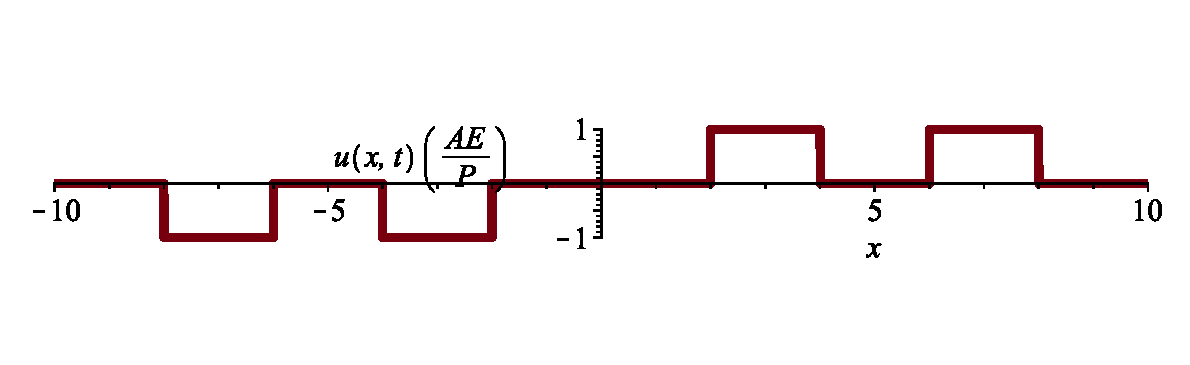
\includegraphics[width = 0.9\textwidth ]{figures/b_u.eps}
    \caption{Case $P H(t)$: Normalized longitudinal displacement along the beam coordinate at $t = 1$s ($L$ and $c$ are equal to 1). Number of terms in the series is 6.}
    \label{fig:b_u}
\end{figure}

\begin{figure}[H]
    \centering
    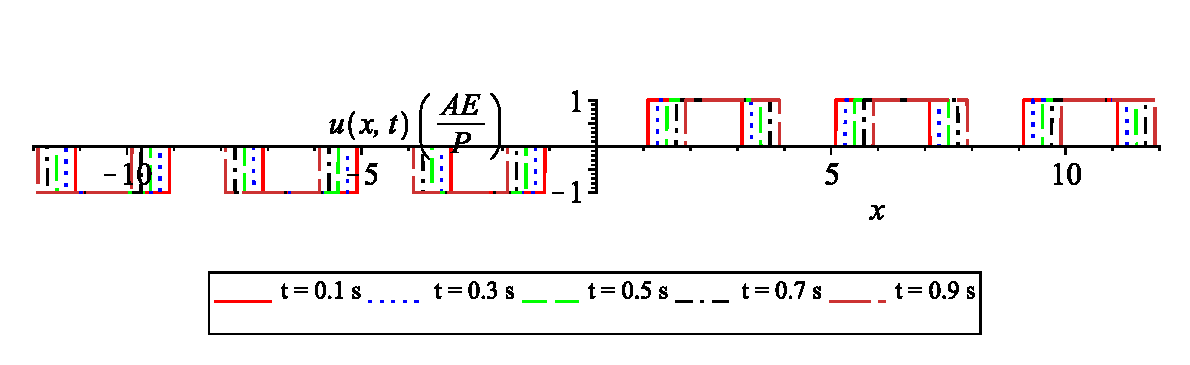
\includegraphics[width = 0.9
    \textwidth ]{figures/b_u_diff_time_inc.eps}
    \caption{Case $P H(t)$: Normalized longitudinal displacement along the beam coordinate for various time increments ($L$ and $c$ are equal to 1). Number of terms in the series is 6.}
    \label{fig:b_u_diff_time_inc}
\end{figure}

\subsubsection{Using $\sinh$ and $\cosh$}
In this section, we continue the solution from \cref{eq:b_laplace_sch} without replacing $\sinh$ and $\cosh$ terms with their equivalent definitions. The Laplace inverse of \cref{eq:b_laplace_sch} can be written as \cite{Spiegel1965}

\begin{equation}
    u(x, t) = \mathcal{L}^{-1}\{ U(x, s) \} = \frac{P(t) c}{AE} \left[ x + \frac{8L}{\pi^2} \sum_{n = 1}^{\infty} \frac{(-1)^n}{(2n - 1)^2} \sin \left( \frac{(2n-1)\pi}{2L}x\right) \cos \left( \frac{(2n-1)\pi}{2L}t\right) \right]
    \label{eq:c_response}
\end{equation}

The response of \cref{eq:c_response} is plotted in \cref{fig:c_u}. This response gives the mode shapes.

\begin{figure}[H]
    \centering
    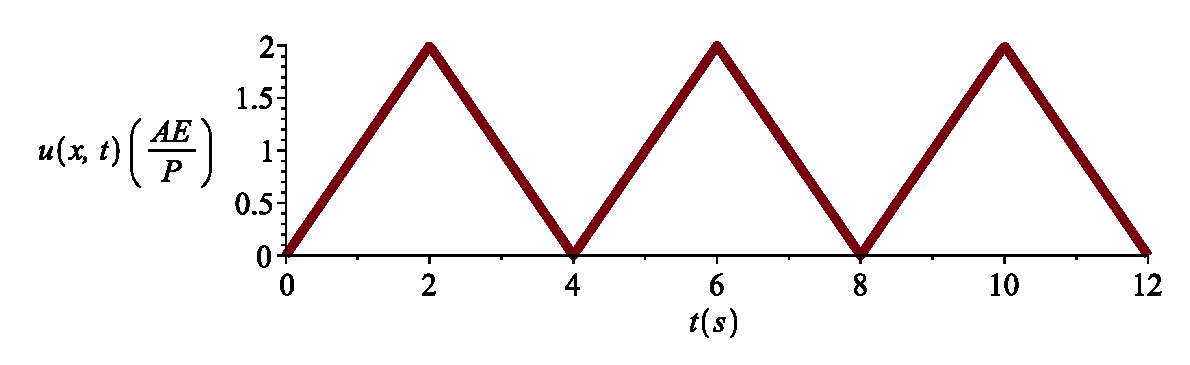
\includegraphics[width = 0.9\textwidth ]{figures/c_u.eps}
    \caption{Case $P H(t)$: Normalized longitudinal displacement for different time increments ($L$, $c$ and $x$ are equal to 1). Number of terms in the series is 1000.}
    \label{fig:c_u}
\end{figure}

\subsubsection{Discussion on Two Approaches of Laplace Transforms}
Let us call the result from Taylor expansion of $\dfrac{1}{1 - x}$ (\cref{eq:b_response}), the series solution and the result from hyperbolic functions (\cref{eq:c_response}), hyperbolic. As mentioned, both results represent two fundamentally-different physical concepts explained earlier in each section. Here, some other aspects are discussed. Since most of the series solution includes Heaviside terms, the series solution procedure is cheaper than the hyperbolic solution in terms of computational cost. Furthermore, the series solution converges much faster than the hyperbolic response. This is well-demonstrated in \cref{fig:c_diff_time_inc} as it requires at least 100 terms in the infinite series of hyperbolic solution to produce an acceptable result. \\

\begin{figure}[H]
        \begin{subfigure}{1\textwidth}
            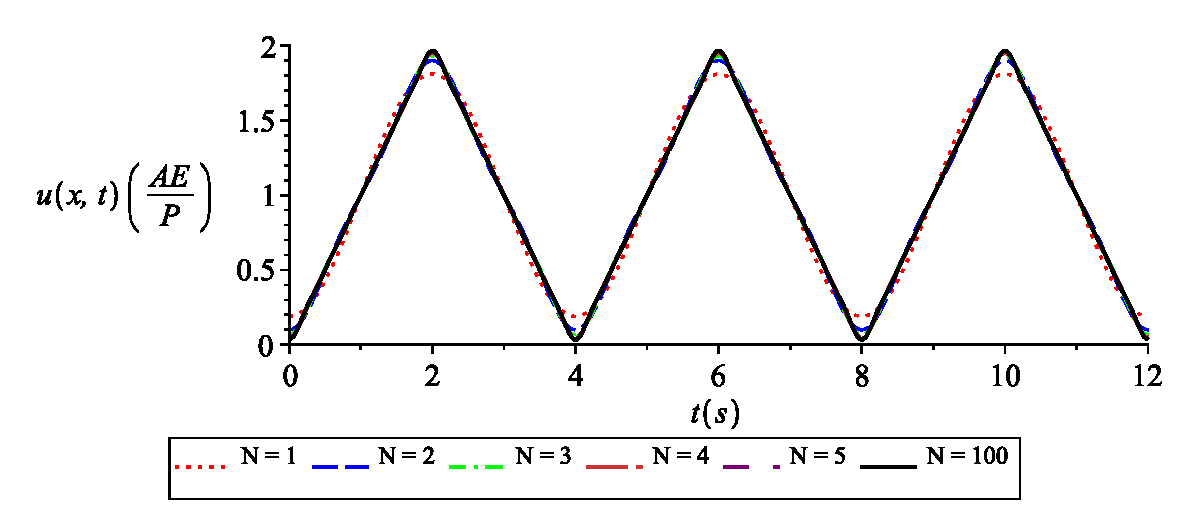
\includegraphics[width=0.9\columnwidth]{figures/c_u_diff_time_inc.eps} 
            \caption{}
            % \label{}
        \end{subfigure}
        \begin{subfigure}{1\textwidth}
            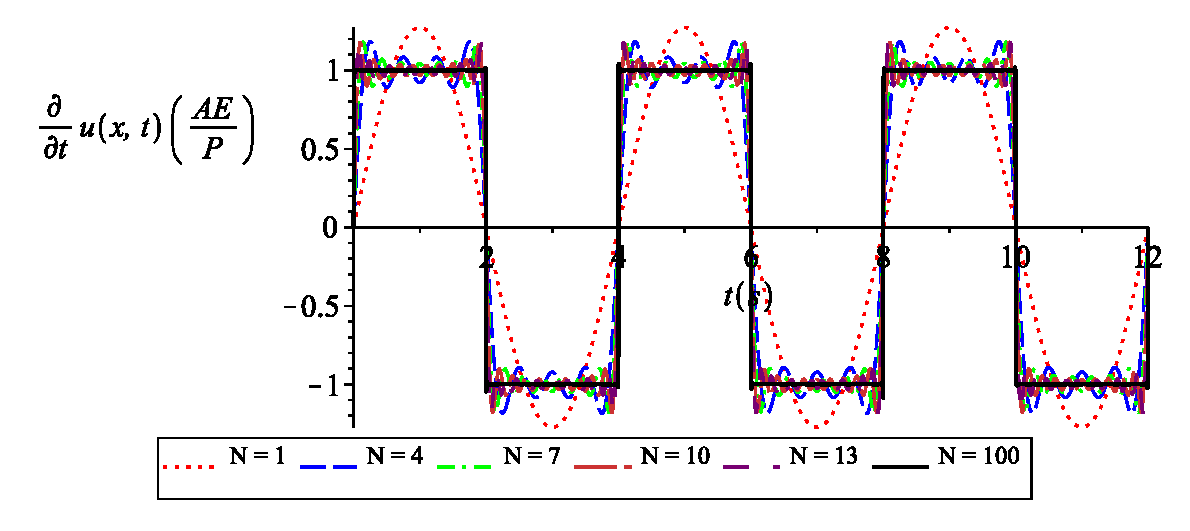
\includegraphics[width=0.9\columnwidth]{figures/c_dudt_diff_time_inc.eps} 
            \caption{}
            % \label{}
        \end{subfigure}
    \caption{Case $P H(t)$: Normalized (a) longitudinal displacement and (b) velocity for different time increments ($L$, $c$ and $x$ equal to 1). $N$ indicates the number of terms in the series.}
    \label{fig:c_diff_time_inc}
\end{figure}

Despite the above-mentioned advantages of the series solution, it suffers from a weakness. For longer beam length, the number of terms in the solution should be increased, unless the proper response cannot be produced. \cref{fig:series_sol_weakness} demonstrates this peculiarity for a longer beam where the series solution is not able to provide further results due to insufficient number of terms in the series. 
\begin{figure}[H]
    \centering
    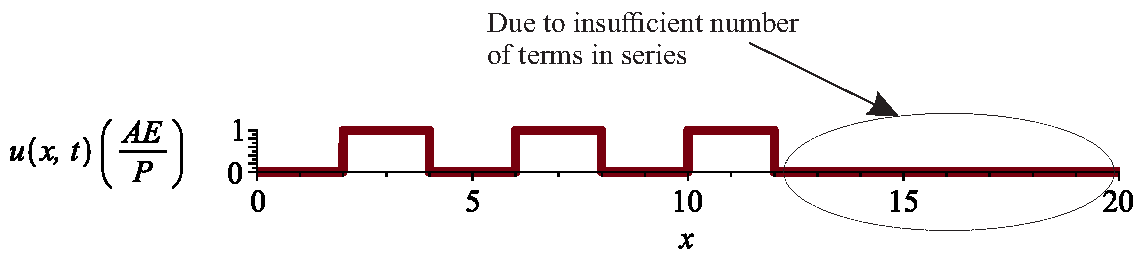
\includegraphics[width = 0.9\textwidth ]{figures/b_u_diff_time_inc_weakness.pdf}
    \caption{The series solution (\cref{eq:b_response}) depends on the number of terms in the infinite series solution and is directly connected with the beam length. Insufficient number of terms does not produce the desired plot (negative part is disregarded in the plot).}
    \label{fig:series_sol_weakness}
\end{figure}




\newpage
\bibliography{ref}
\bibliographystyle{ieeetr}

\end{document}